A continuación se presenta un diagrama gerárquico, el cual muestra los
objetivos a lograr, los cuales son descompuestos en objetivos más pequeños
sucesivamente, hasta lograr llegar a objetivos lo suficientemente pequeños como
para ser asignados a una sola persona o agente capaz de realizarlo.

\begin{center}

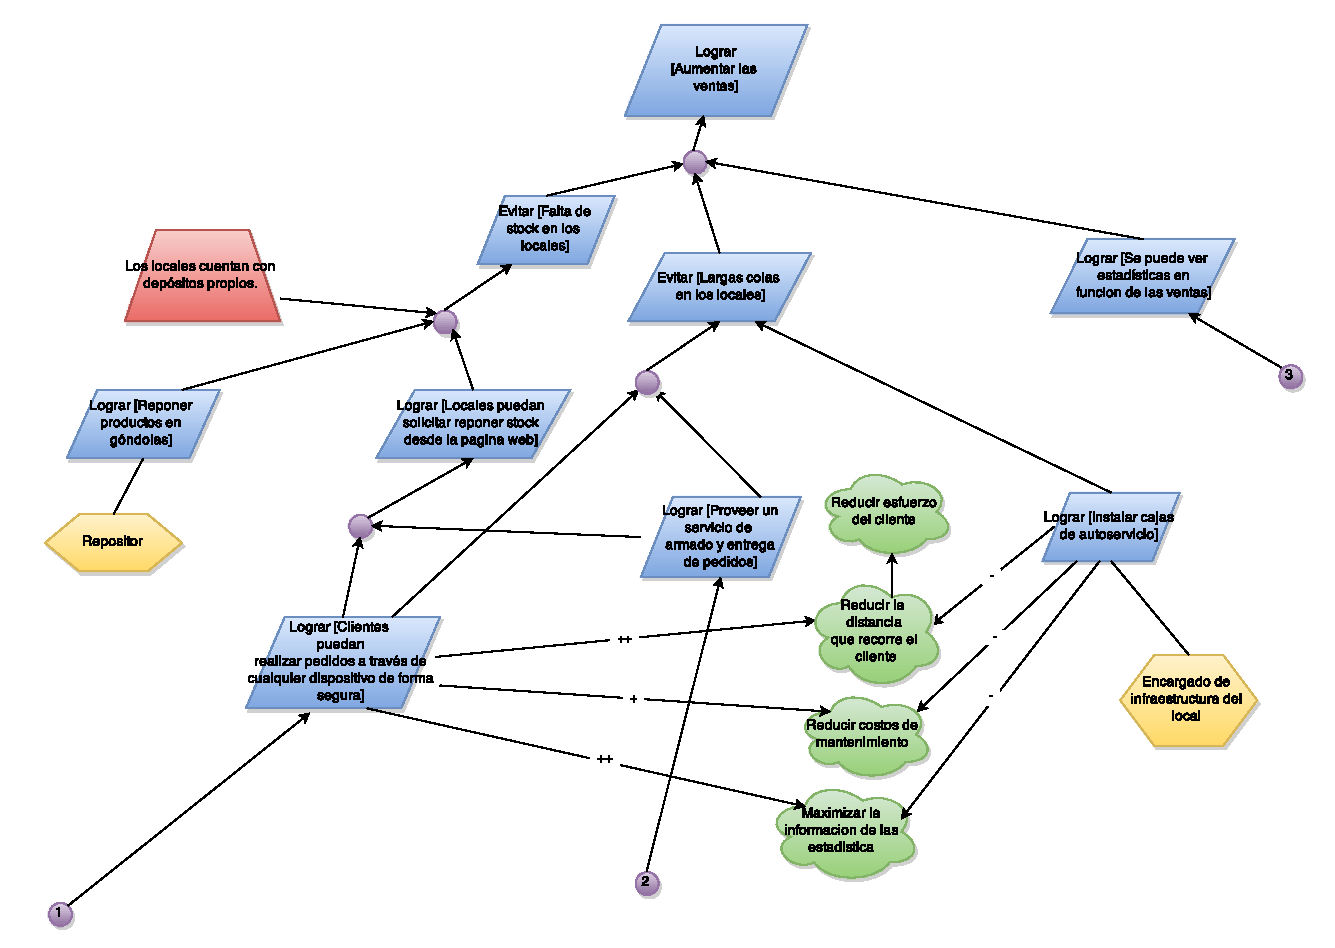
\includegraphics[scale=0.9, angle=90]{diagrama-de-objetivos-split-0}
\newpage
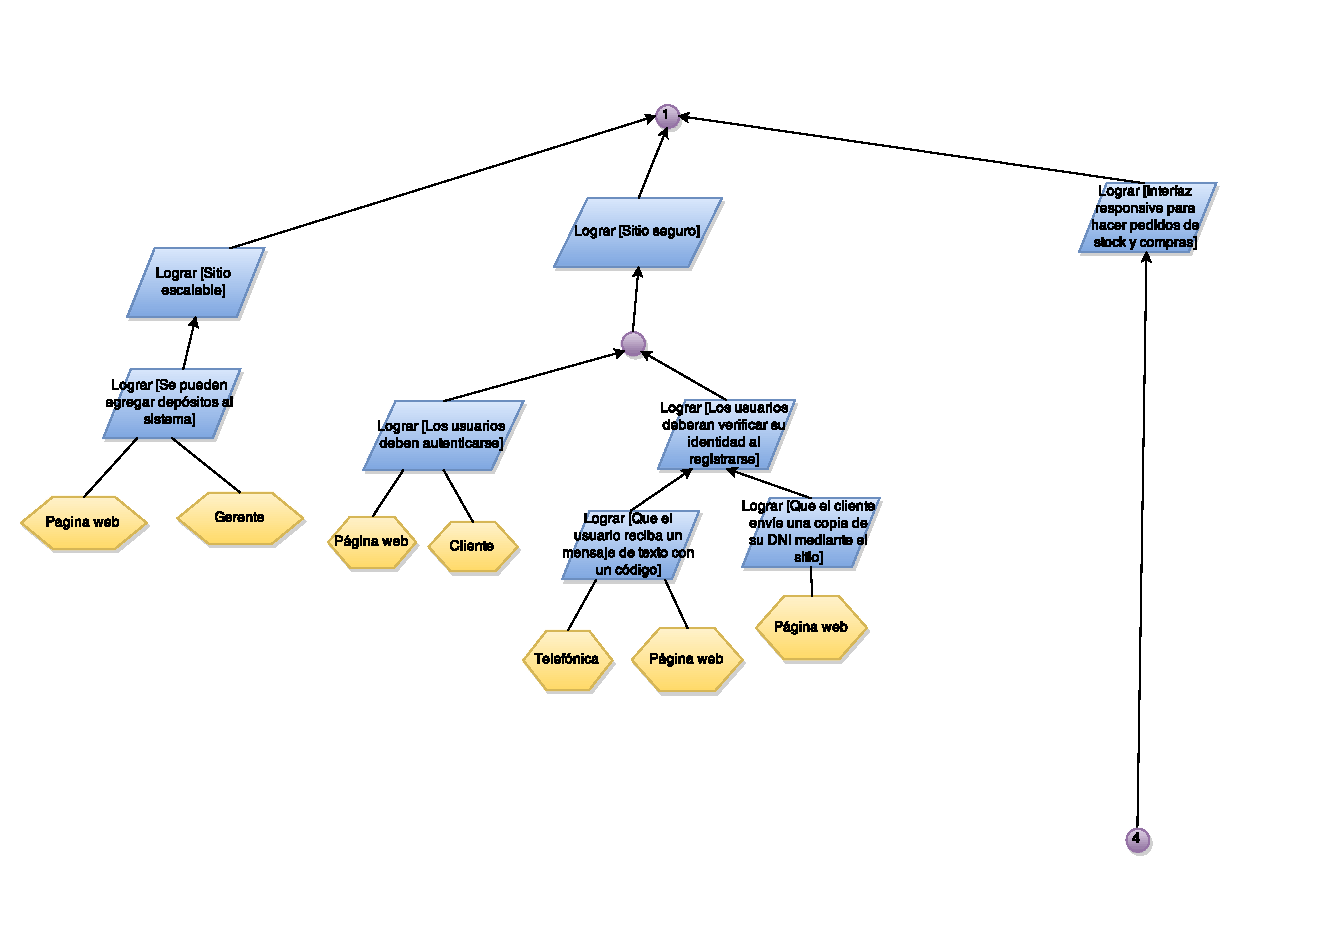
\includegraphics[scale=0.9, angle=90]{diagrama-de-objetivos-split-1}
\newpage
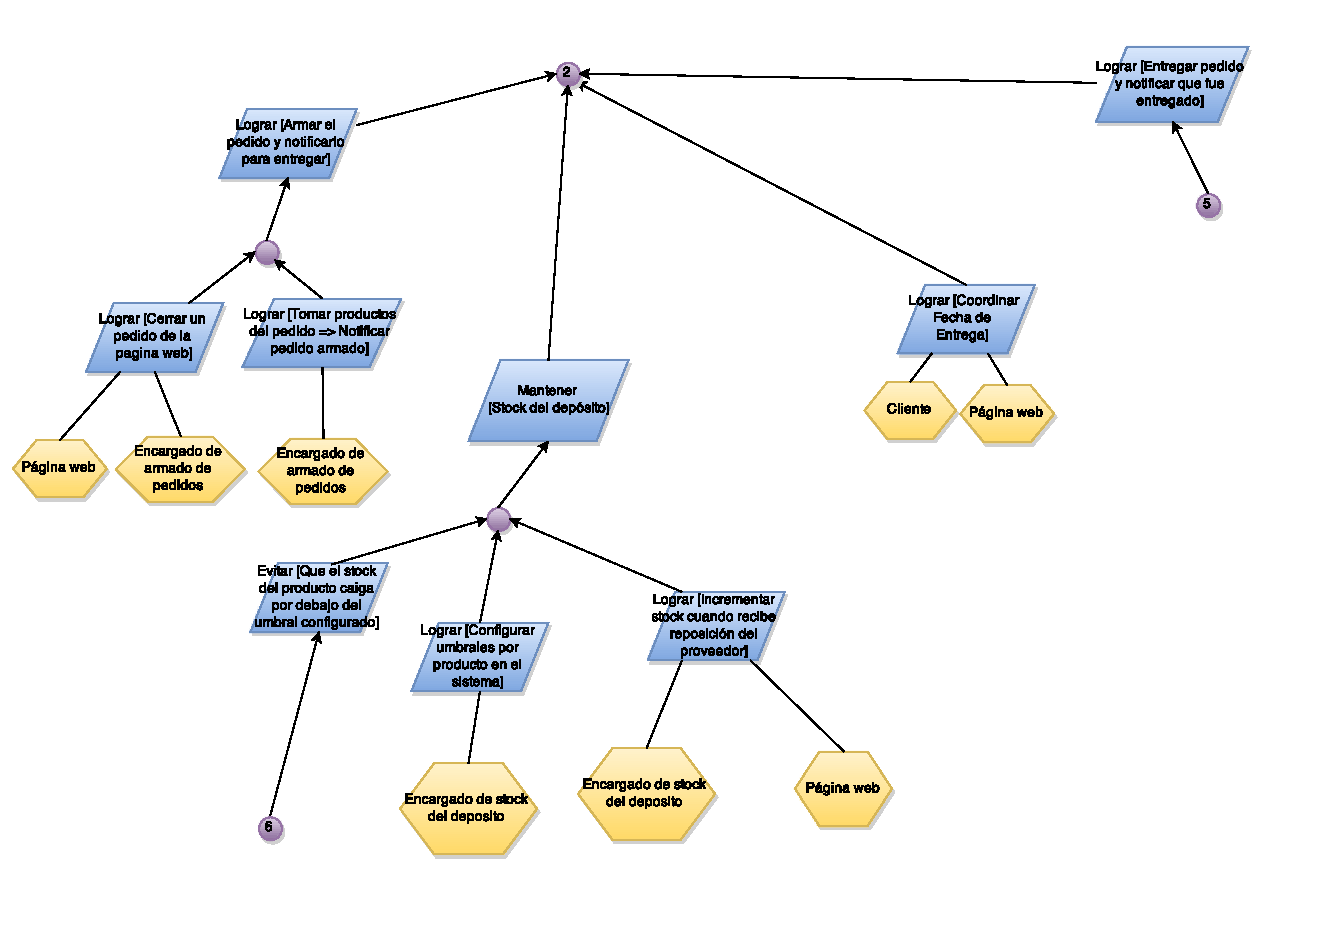
\includegraphics[scale=0.9, angle=90]{diagrama-de-objetivos-split-2}
\newpage
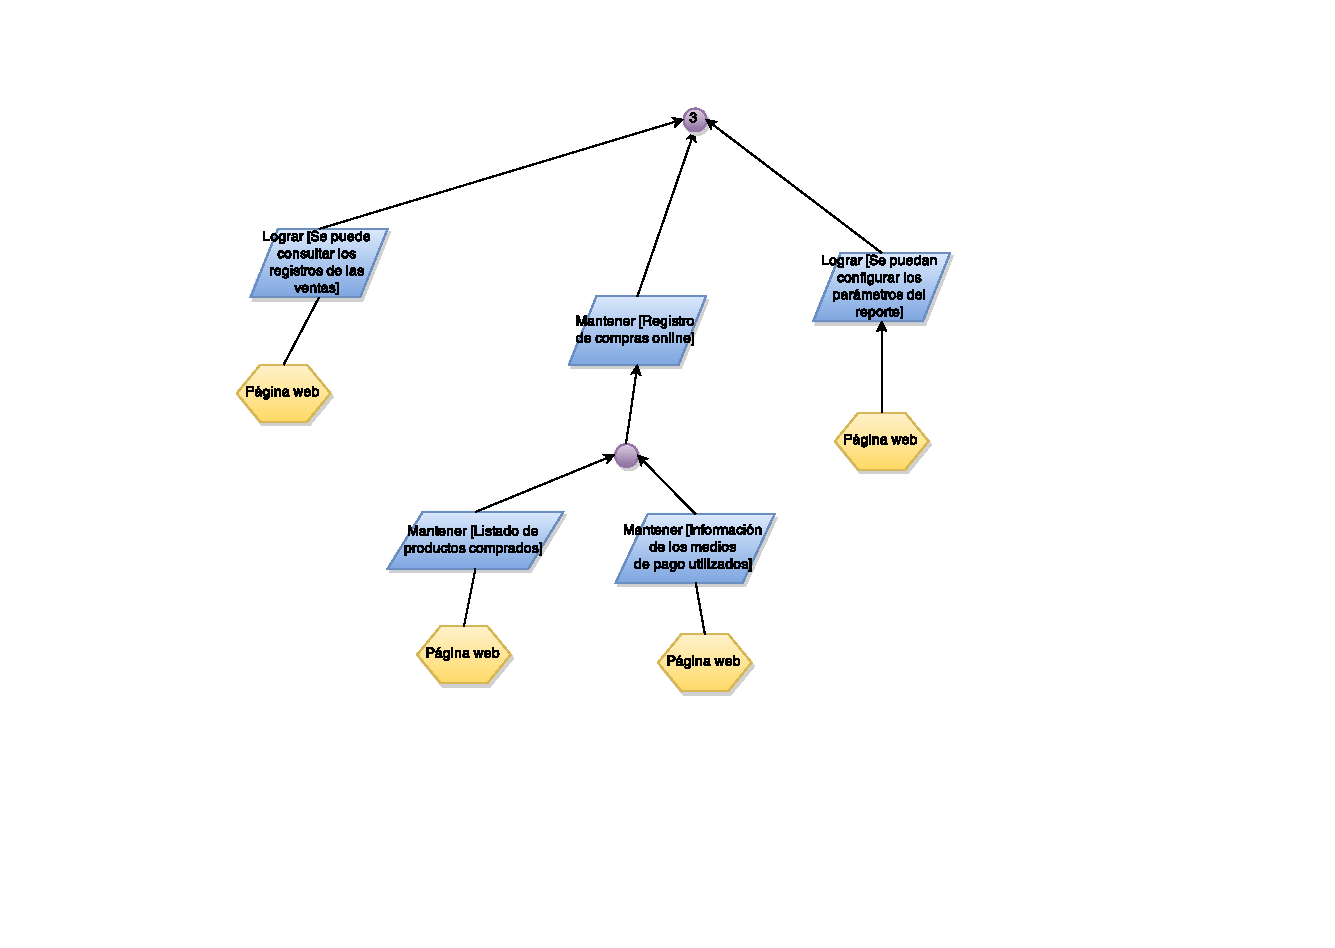
\includegraphics[scale=0.9, angle=90]{diagrama-de-objetivos-split-3}
\newpage
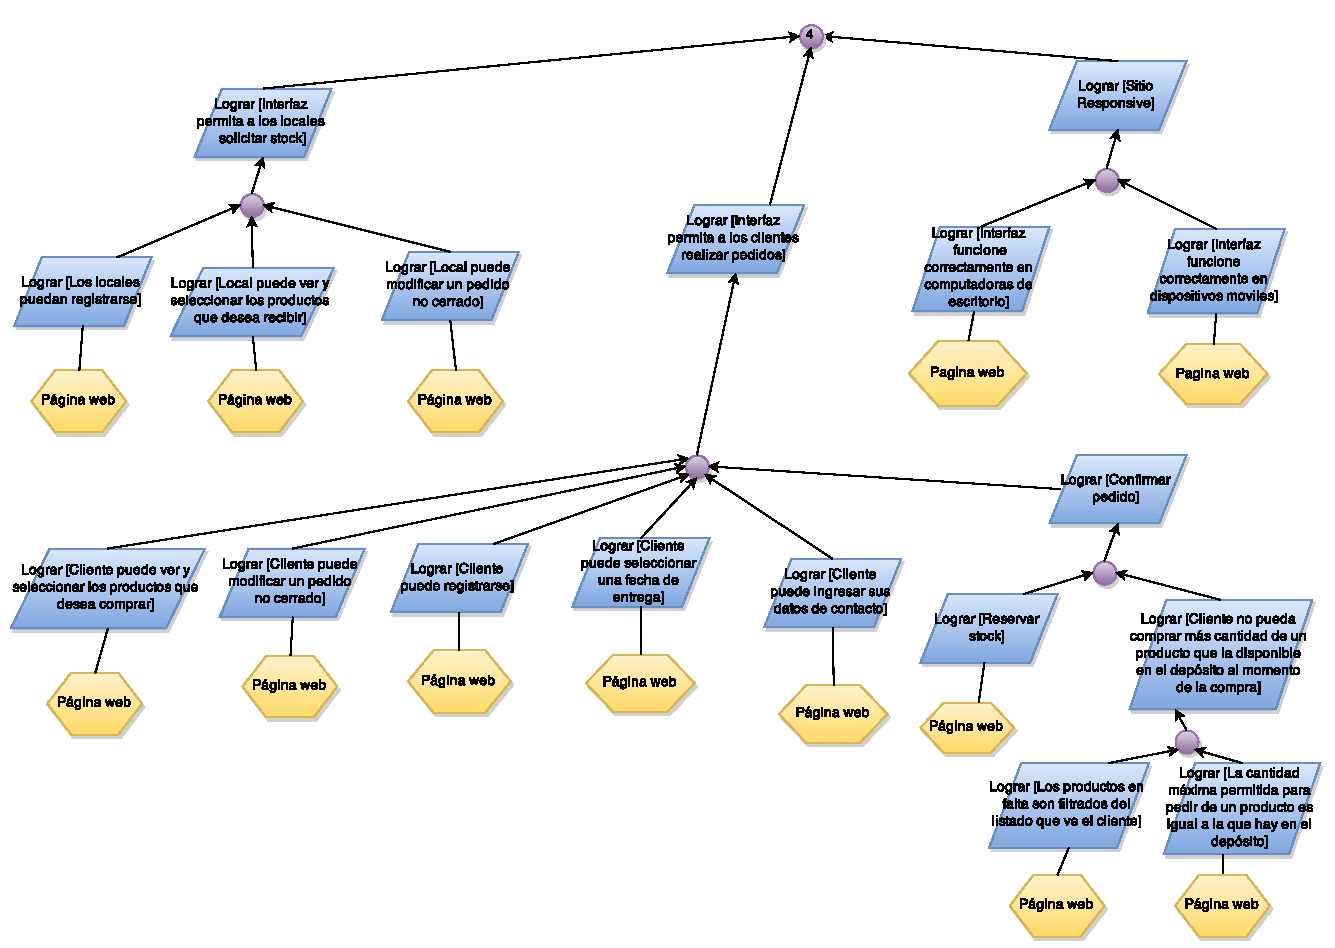
\includegraphics[scale=0.9, angle=90]{diagrama-de-objetivos-split-4}
\newpage
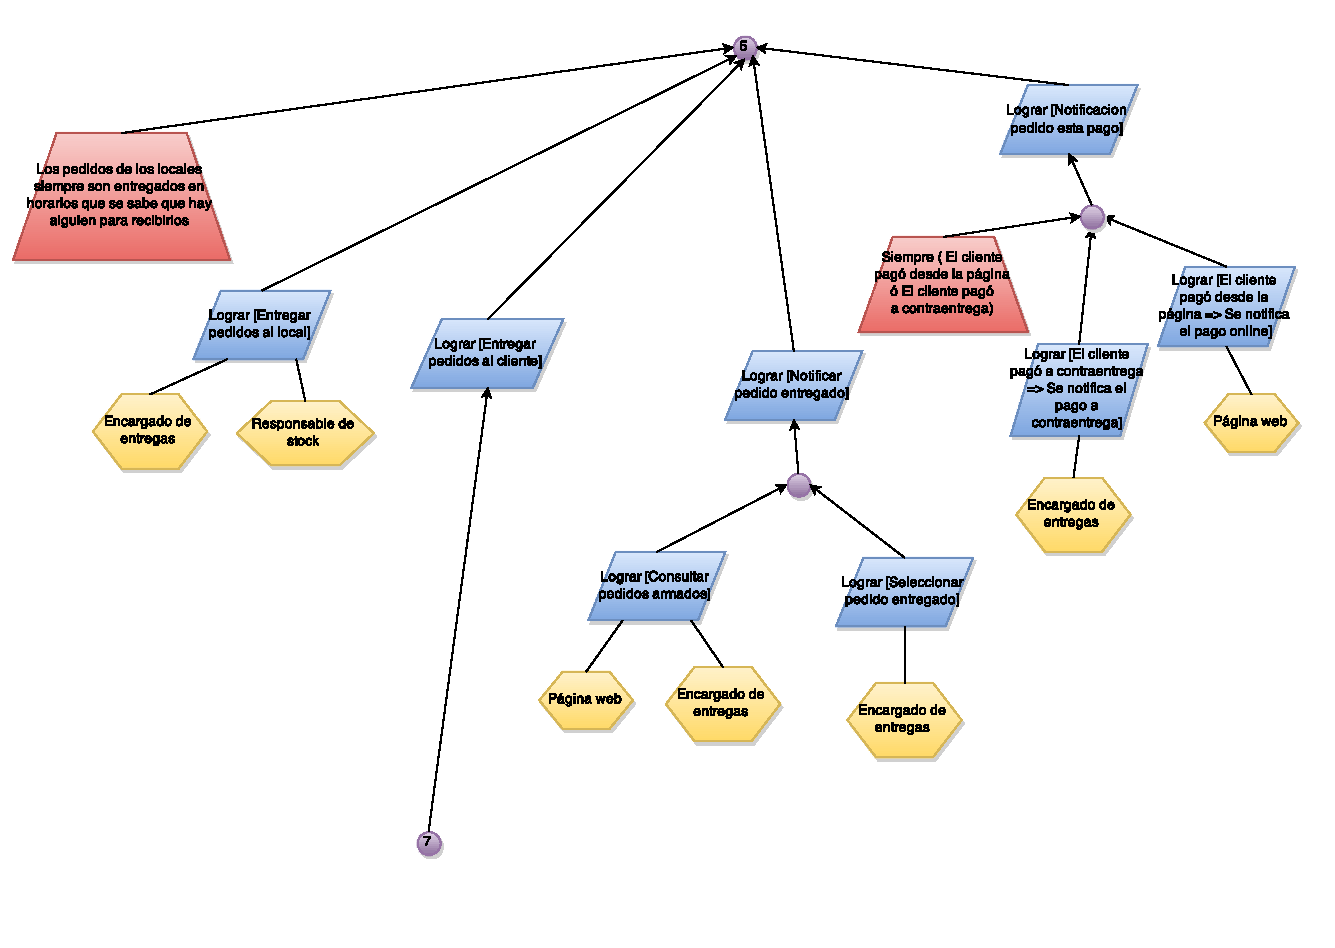
\includegraphics[scale=0.9, angle=90]{diagrama-de-objetivos-split-5}
\newpage
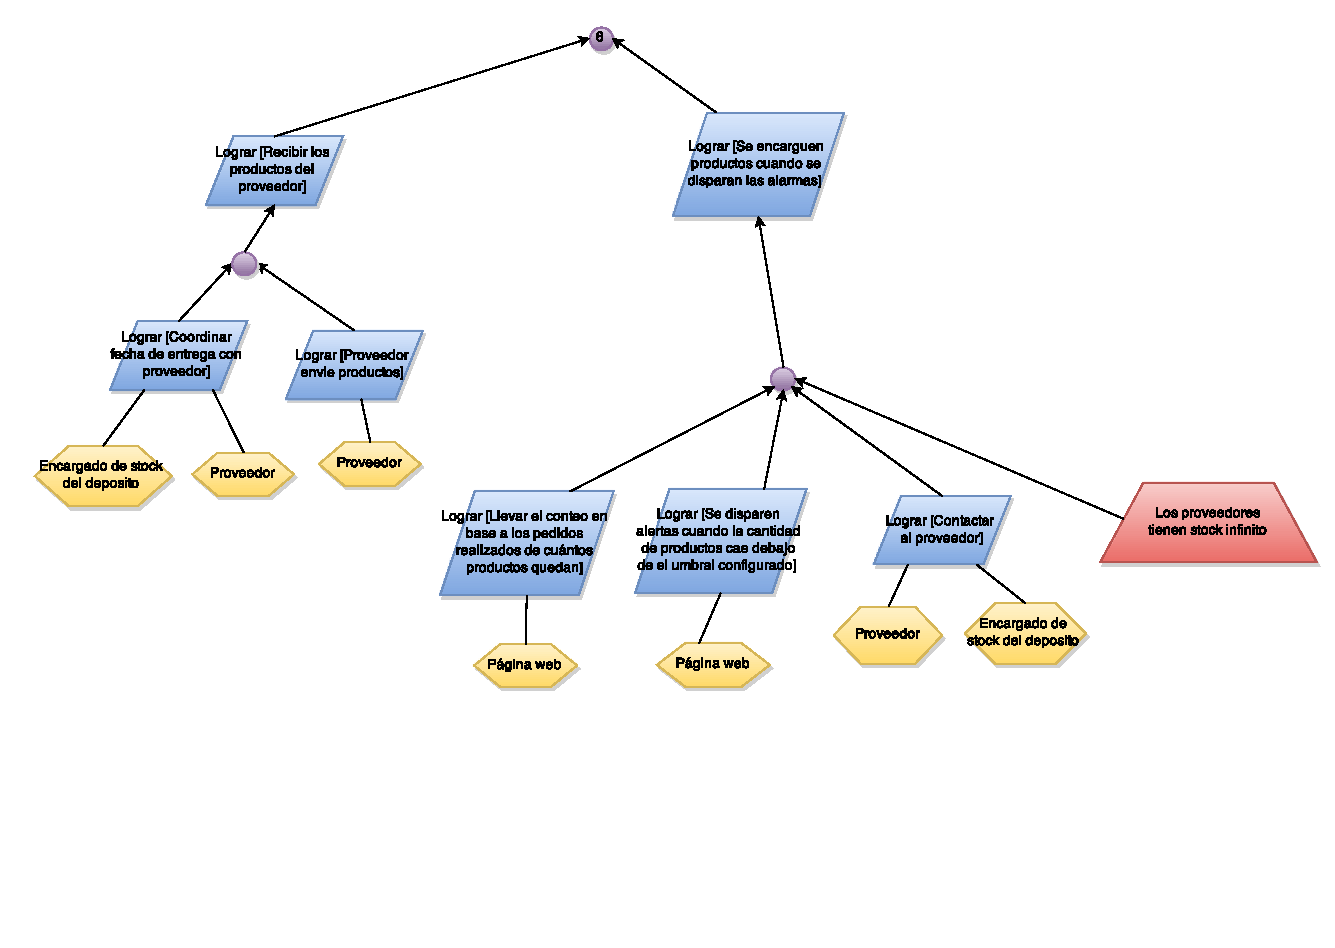
\includegraphics[scale=0.9, angle=90]{diagrama-de-objetivos-split-6}
\newpage
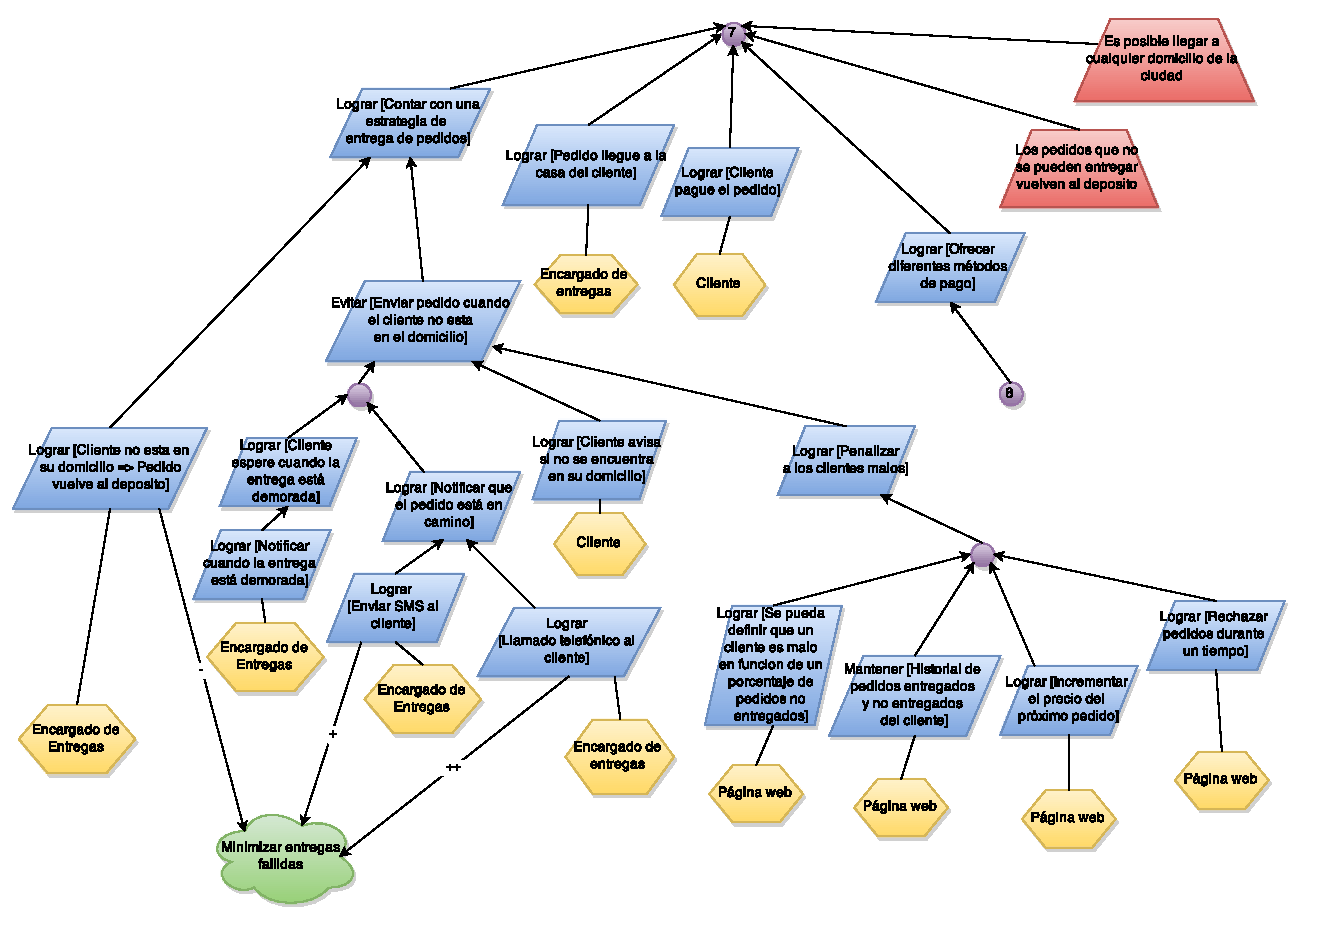
\includegraphics[scale=0.9, angle=90]{diagrama-de-objetivos-split-7}
\newpage
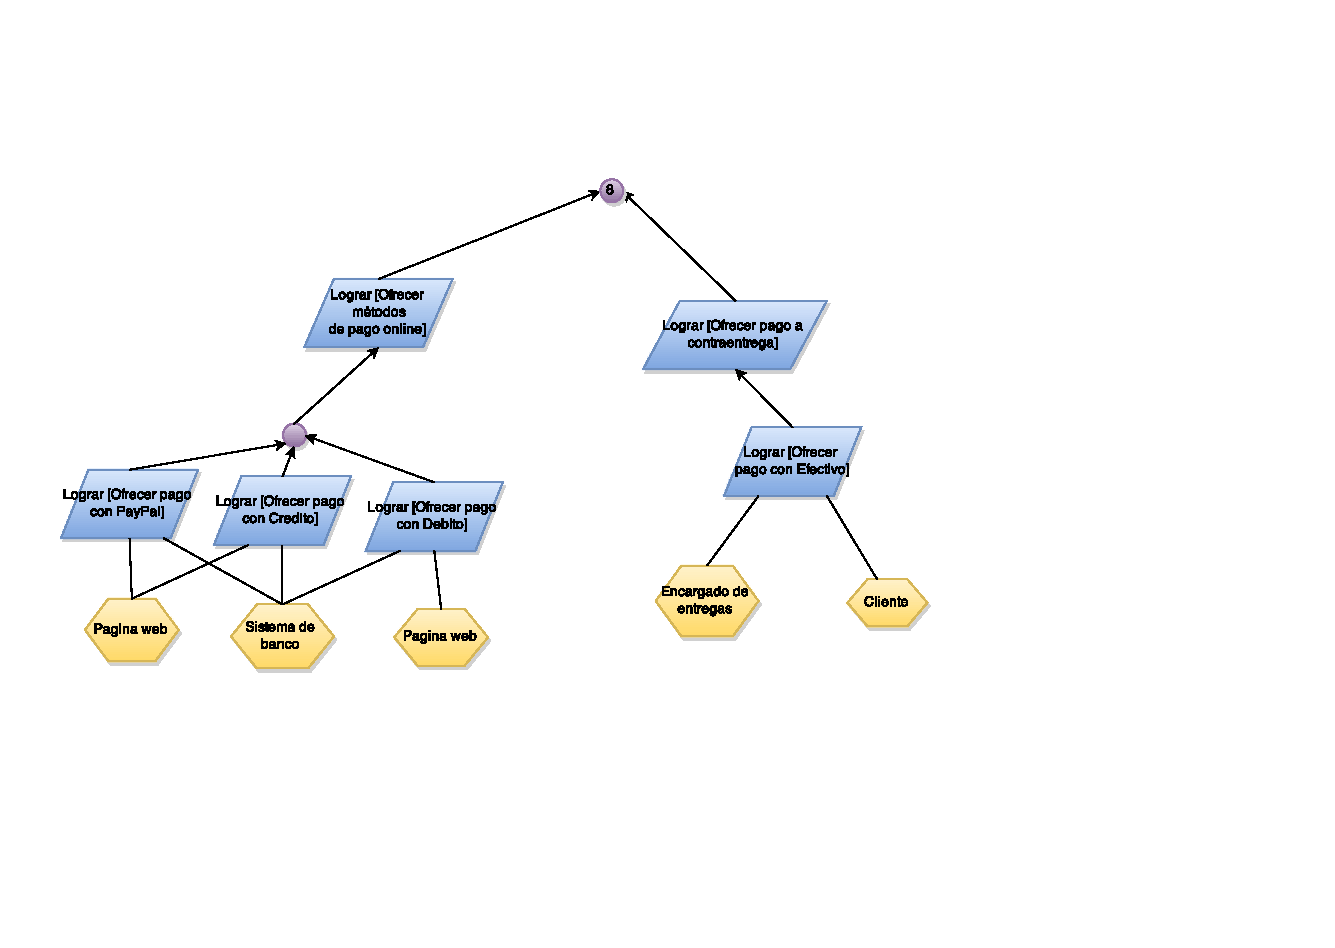
\includegraphics[scale=0.9, angle=90]{diagrama-de-objetivos-split-8}
\newpage

\begin{longtable}{p{7cm} p{7cm}}
\textbf{Objetivo} & \textbf{Descripción} \\[0.2em] \hline
\endhead

Lograr [\textit{Aumentar las ventas}] & Aumentar las ventas en los locales de \textbf{Mes\%}. \\[0.2em] \hline

Evitar [\textit{Falta de stock en los locales}] & Evitar que falten productos en las góndolas. \\[0.2em] \hline

Evitar [\textit{Largas colas en los locales}] & Evitar que haya excesivo tiempo de espera en las colas de las cajas. \\[0.2em] \hline

Lograr [\textit{Se puede ver estadísticas en función de las ventas}] & Mostrar información interesante a partir de los datos provistos por las ventas realizadas a través de la página web para que el gerente pueda tomar mejores decisiones estratégicas. \\[0.2em] \hline

Mantener [\textit{Registro de compras online}] &  Cada vez que se hace una compra (ya sea una compra de un cliente o un pedido de reposición de stock de un local) a través de la página web se almacenan en el sistema los productos comprados y los métodos de pago utilizados. \\[0.2em] \hline

Mantener [\textit{Información de los medios de pago utilizados}] & El sistema almacena información referente a la forma de pago elegida (online o contra-entrega) y al método de pago (crédito, débito o efectivo), además del monto pagado. \\[0.2em] \hline

Mantener [\textit{Listado de productos comprados}] & El sistema almacena información referente a el tipo de productos comprados y a la cantidad de cada uno de ellos. \\[0.2em] \hline

Lograr [\textit{Sistema para realizar pedidos de forma remota}] & Las reposiciones de stock de los locales y los pedidos de los cliente se realizan a través de un sistema remoto, de modo que estos pueden encargar productos sin salir de su casa. \\[0.2em] \hline

Lograr [\textit{Instalar cajas de autoservicio}] & Se instalan cajas en donde el cliente puede colocar sus productos y registrarlos él mismo. Luego tiene que pagarlos con una cajera. \\[0.2em] \hline

Lograr [\textit{Locales puedan solicitar reponer stock desde la página Web}] & La página pueda recibir solicitudes de reponer stock de un local. \\[0.2em] \hline

Lograr [\textit{Clientes puedan realizar pedidos a través de cualquier dispositivo de forma segura}] & La página recibe pedidos de clientes y los datos no se pierden, no los intercepta un tercero y la información relevante para el cliente está disponible en la página. \\[0.2em] \hline

Lograr [\textit{Proveer un servicio de armado y entrega de pedidos}] & Luego de que el cliente realiza un pedido en la página, este es confirmado, armado y enviado a su domicilio. \\[0.2em] \hline

Lograr [\textit{Armar el pedido y notificarlo para entregar}] & Luego de que un cliente hace un pedido, se procede a buscar los productos del pedido, se lo arma y se notifica que este ya esta terminado. \\[0.2em] \hline

Lograr [\textit{Obtener un pedido de la página web}] & El encargado de armado de pedidos debe ingresar a la página web y cerrar el pedido que comenzará a armar. \\[0.2em] \hline

Lograr [\textit{Proveer un sitio Web escalable, seguro y responsive para realizar pedidos}] & Los pedidos de los clientes se hacen de forma segura y el usuario puede verlos tanto en un navegador estándar como en un dispositivo móvil, además se pueden colocar más depósitos en el sistema y configurarlos. \\[0.2em] \hline

Lograr [\textit{Tomar productos del pedido => Notificar pedido armado}] & El encargado de armado de pedidos debe tomar del stock a todos los productos que se encuentran en el pedido y, una vez que haya terminado, deberá notificar al encargado de entregas que el pedido ya fue armado y esta listo para ser entregado. \\[0.2em] \hline

Mantener [\textit{Stock del depósito}] & Se debe mantener el stock de cada producto del depósito, de manera que cuando haya un pedido éste pueda ser cumplido sin problemas. \\[0.2em] \hline

Evitar [\textit{Stock del producto caiga por debajo del umbral configurado}] & Se debe contactar al proveedor y encargarle más unidades del producto del cual hay poco stock antes de que este se agote o haya una cantidad insuficiente para un pedido. \\[0.2em] \hline

Lograr [\textit{Recibir los productos del proveedor}] & El encargado del stock del deposito debera recibir los productos enviados por el proveedor en la fecha acordada previamente. \\[0.2em] \hline

Lograr [\textit{Coordinar fecha de entrega con proveedor}] & El encargado del stock del depósito y el proveedor deben ponerse de acuerdo sobre la fecha en que el pedido será entregado en el depósito. \\[0.2em] \hline

Lograr [\textit{Proveedor envíe productos}] & El proveedor debe enviar todos los productos encargados en la fecha acordada. \\[0.2em] \hline

Lograr [\textit{Se encarguen productos cuando se disparan las alarmas}] & Cuando la página web avise que un producto escasea se debe contactar al proveedor para que éste envíe más unidades del producto en cuestión. \\[0.2em] \hline

Lograr [\textit{Llevar el conteo en base a los pedidos realizados de cuántos productos quedan}] & Cada vez que se cierra un pedido la página web actualizará el stock de los productos utilizados para completar dicho pedido. \\[0.2em] \hline

Lograr [\textit{Se disparan alertas cuando la cantidad de productos cae debajo del umbral configurado}] & Cuando el stock de un producto caiga por debajo de un valor determinado, la página web enviará una alerta al encargado del depósito para que éste reponga su stock. \\[0.2em] \hline

Lograr [\textit{Contactar al proveedor}] & Comunicarse con el proveedor para encargar productos. \\[0.2em] \hline

Lograr [\textit{Configurar umbrales por producto en el sistema}] & Por cada producto del sistema asignarle un valor para el cual, si el stock del producto cae por debajo de dicho valor, entonces se envía una alerta de reponer el stock de dicho producto. \\[0.2em] \hline

Lograr [\textit{Coordinar Fecha de  Entrega}] & Se acuerda una fecha con el depósito para que se envíe el pedido al cliente. \\[0.2em] \hline

Lograr [\textit{Penalizar a los clientes malos}] & Se penaliza un cliente por no estar en su domicilio. \\[0.2em] \hline

Lograr [\textit{Se pueda definir que un cliente es malo en función de un porcentaje de pedidos no entregados}] & La página web permite definir cuando un cliente es considerado un “mal cliente”, en función del porcentaje de pedidos que no pudieron ser entregados sobre la cantidad de pedidos totales. \\[0.2em] \hline

Mantener [\textit{Historial de pedidos entregados y no entregados del cliente}] & Se debe guardar un historial por cada cliente en donde se encuentran los pedidos entregados y no entregados. \\[0.2em] \hline

Lograr [\textit{Penalizar al cliente}] & Se puede penalizar a un cliente cuando éste no está en su domicilio a la hora de la entrega. \\[0.2em] \hline

Lograr [\textit{Rechazar pedidos durante un tiempo}] & Una de las formas de penalizar a un cliente por no estar en la casa es rechazando sus pedidos de compra durante un tiempo (a configurar por la gerencia). \\[0.2em] \hline

Lograr [\textit{Incrementar el precio del proximo pedido}] & Se incrementa el precio (en una cantidad o porcentaje configurable) del próximo pedido que el cliente realice como forma de castigo por no haber estado en su domicilio cuando se le envió un pedido. \\[0.2em] \hline

Lograr [\textit{Entregar pedido y notificar que fue entregado}] & Se consigue entregar el pedido y se notifica que el pedido fue entregado correctamente. \\[0.2em] \hline

Lograr [\textit{Notificación pedido está pago}] & Se notifica en la página que el pedido se pagó correctamente. \\[0.2em] \hline

Lograr [\textit{El cliente pagó desde la página => Se notifica el pago online}] & Si el pago se realiza por la página web, entonces se notifica al cliente y/o encargados en el depósito de su pago. \\[0.2em] \hline

Lograr [\textit{El cliente pagó a contraentrega => Se notifica el pago a contraentrega}] & En la página se puede notificar que el pago es a contraentrega. \\[0.2em] \hline

Lograr [\textit{Notificar pedido entregado}] & En la página se puede notificar que el pedido ha sido entregado. \\[0.2em] \hline

Lograr [\textit{Entregar pedidos al cliente}] & El pedido se entrega al cliente. \\[0.2em] \hline

Lograr [\textit{Contar con una estrategia de entrega de pedidos}] & Tener un procedimiento para entregar un pedido. \\[0.2em] \hline

Lograr [\textit{Cliente no está en su domicilio => Pedido vuelve al depósito}] & Si el cliente no está en el domicilio entonces el pedido debe volver al depósito. \\[0.2em] \hline

Evitar [\textit{Enviar pedido cuando el cliente no está en el domicilio}] & Mantener al cliente en el domicilio cuando se realiza una entrega. \\[0.2em] \hline

Lograr [\textit{Cliente espere cuando la entrega está demorada}] & Si el pedido está demorado que el cliente espere. \\[0.2em] \hline

Lograr [\textit{Notificar cuando la entrega está demorada}] & El encargado de entregas notifica que la entrega está demorada. \\[0.2em] \hline

Lograr [\textit{Notificar que el pedido está en camino}] & El encargado de entregas notifica que el producto salió del depósito rumbo a su domicilio. \\[0.2em] \hline

Lograr [\textit{Enviar SMS al cliente}] & Se envía un SMS al cliente para avisar que el pedido esta en camino. \\[0.2em] \hline

Lograr [\textit{Llamado telefónico al cliente}] & Se llama al cliente para avisar que el pedido esta en camino. \\[0.2em] \hline

Lograr [\textit{Cliente avisa si no se encuentra en su domicilio}] & El cliente puede avisar que no se encuentra en el domicilio para evitar entregarlo sin que este. \\[0.2em] \hline

Lograr [\textit{Pedido llegue a la casa del cliente}] & El transporte puede llegar a la casa del cliente. \\[0.2em] \hline

Lograr [\textit{Ofrecer diferentes métodos de pago}] & Que la página web provea diferentes métodos de pago. \\[0.2em] \hline

Lograr [\textit{Ofrecer métodos de pago online}] & Que la página web provea pago online. \\[0.2em] \hline

Lograr [\textit{Ofrecer pago con PayPal}] & El pago se realiza mediante PayPal. \\[0.2em] \hline

Lograr [\textit{Ofrecer pago con Crédito}] & El pago se realiza mediante una tarjeta de crédito. \\[0.2em] \hline

Lograr [\textit{Ofrecer pago a contraentrega}] & El pago se realiza en el domicilio. \\[0.2em] \hline

Lograr [\textit{Ofrecer pago con Efectivo}] & El cliente paga en efectivo. \\[0.2em] \hline

Lograr [\textit{Entregar pedidos al local}] & Las solicitudes de reponer stock se entregan al local. \\[0.2em] \hline

Lograr [\textit{Proveer un sitio web escalable, seguro y responsive para realizar pedidos}] & Los pedidos de los clientes se hacen de forma segura y el usuario puede verlos tanto en un navegador estándar como en un dispositivo móvil, además se pueden agregar más depósitos en el sistema. \\[0.2em] \hline

Lograr [\textit{Sitio escalable}] & El sitio ofrece la posibilidad de agregar nuevos depósitos. \\[0.2em] \hline

Lograr [\textit{Se pueden agregar depósitos al sistema}] & El sistema permite añadir más depósitos. \\[0.2em] \hline

Lograr [\textit{Sitio seguro}] & Tener seguridad en el sistema, tanto en el logeo como a la hora de hacer los pedidos. \\[0.2em] \hline

Lograr [\textit{Los usuarios deberán verificar su identidad al registrarse}] & Para verificar que el usuario que se registra es una persona real y no es otra persona ya registrada. \\[0.2em] \hline

Lograr [\textit{Los usuarios deben autenticarse}] & Con fines de que ningún usuario se haga pasar por otro, se requiere que cada cliente se loguee con su usuario y contraseña. Este logeo se hace desde la página Web. \\[0.2em] \hline

Lograr [\textit{Que el usuario reciba un mensaje de texto con un código}] & Cuando se registra indicando en sus datos de contacto su número de celular, recibe una confirmación con un código en un sms para que lo ingrese en la página y pueda confirmar su registro. \\[0.2em] \hline

Lograr [\textit{Que el cliente pueda enviar una copia de su DNI mediante el sitio}] & El sitio permite al cliente enviar una imagen (escaneo del DNI), para que así éste pueda confirmar su identidad y su usuario sea dado de alta. \\[0.2em] \hline

Lograr [\textit{Interfaz responsive necesaria para locales y clientes}] & Se debe construir una interfaz web que se adapte tanto a los dispositivos móviles como a las computadoras de escritorio que permite a los clientes realizar pedidos y a los locales solicitar reposición de stock. \\[0.2em] \hline

Lograr [\textit{Interfaz permite a los locales solicitar stock}] & Un local, desde la página, podrá enviar solicitudes para reponer su stock. \\[0.2em] \hline

Lograr [\textit{Cada local tenga un usuario}] & Cada local deberá tener un usuario distinto en el sitio web para poder realizar sus pedidos. \\[0.2em] \hline

Lograr [\textit{Local puede ver y seleccionar los productos que desea recibir}] & Al realizar un pedido de reposición de stock se podrá ver los productos disponibles y seleccionar aquellos que se deseen. \\[0.2em] \hline

Lograr [\textit{Local puede modificar un pedido no cerrado}] & Mientras un pedido no haya sido marcado como cerrado, el local podrá añadir, quitar y modificar la cantidad de productos encargados. \\[0.2em] \hline

Lograr [\textit{Interfaz permita a los clientes realizar pedidos}] & Los clientes podrán realizar pedidos de productos a través de la página web. \\[0.2em] \hline

Lograr [\textit{Cliente puede ver y seleccionar los productos que desea comprar}] & Cuando un cliente desea realizar un pedido podrá ver todos los productos que hay disponibles y seleccionar aquellos que desea comprar. \\[0.2em] \hline

Lograr [\textit{Cliente puede modificar un pedido no cerrado}] & Mientras un pedido no esté marcado como cerrado, el cliente podrá añadir, quitar y modificar la cantidad de productos encargados. \\[0.2em] \hline

Lograr [\textit{Cliente puede registrarse}] & Al ingresar un usuario y contraseña correctos, el cliente podrá registrarse en el sitio web. \\[0.2em] \hline

Lograr [\textit{Cliente puede seleccionar una fecha de entrega}] & El sitio debe proveer al cliente un listado con las fechas disponibles para enviarle su pedido. \\[0.2em] \hline

Lograr [\textit{Cliente puede ingresar sus datos de contacto}] & Cada cliente puede ingresar sus datos en la página web. \\[0.2em] \hline

Lograr [\textit{Sitio responsive}] & El sitio tiene que ser adaptable para todos los dispositivos y navegadores. \\[0.2em] \hline

Lograr [\textit{Interfaz funcione correctamente en computadoras de escritorio}] & El sitio tiene que funcionar correctamente en computadoras de escritorio, para los navegadores. \\[0.2em] \hline

Lograr [\textit{Interfaz funcione correctamente en dispositivos móviles}] & El sitio tiene que funcionar correctamente en todos los celulares, tablets y smartphones. \\[0.2em] \hline

\end{longtable}
\end{center}
